\section[EL SISTEMA DODECAF\'ONICO DE SCHOENBERG]{EL SISTEMA DODECAF\'ONICO DE SCHOENBERG}\label{ch:dodecafonismo}
	\subsection{Los postulados del dodecafonismo}
		El dodecafonismo es un sistema compositivo que predetermina la melod\'ia y la armon\'ia a partir de una ordenaci\'on de las doce notas de la escala crom\'atica, que se llama \textit{serie}. \'Esta y algunas de sus transformaciones son los ladrillos con los que se construyen las alturas de las notas; son el \'unico material que se puede utilizar. 
		
		El resto de elementos de la pieza, como el n\'umero de instrumentos, el ritmo, el car\'acter, la textura o las din\'amicas, se dejan a discreci\'on del compositor. No serializar todos los conjuntos ser\'a la principal cr\'itica al dodecafonismo por parte de los compositores serialistas que sucedieron a su creador, Arnold Schoenberg. Para los serialistas integrales, como Pierre Boulez, aquello restaba cohesi\'on al modelo compositivo; para los dodecafonistas, aportaba libertad. \cite{boulez}
		
		Precisamente la predeterminaci\'on dodecaf\'onica, aunque parece limitante, permite realizaciones musicales y estilos de composici\'on muy diferentes: Schoenberg daba un tratamiento tradicional a sus obras, ya que a\'un admiraba las formas cl\'asicas; Alban Berg iba m\'as all\'a al utilizar series que recordaban a las tr\'iadas tonales; y, en cambio, Anton Webern evitaba radicalmente cualquier asociaci\'on con la tradici\'on. 
		
		Schoenberg defini\'o su sistema musical a partir de cuatro postulados que, en realidad, se basan en principios matem\'aticos \cite{dominguez}:
		
		\emph{1. La serie \emph{[sobre la que se construye la obra dodecaf\'onica]} consta de las doce notas de la escala crom\'atica dispuestas en un orden lineal espec\'ifico.}
		
		\emph{2. Ninguna nota aparece m\'as de una vez en la serie.}
		
		Los dos primeros postulados expresan que una obra dodecaf\'onica fundamenta su estructura sobre una permutaci\'on de la escala de doce semitonos. Dicha permutaci\'on $\sigma$ es una biyecci\'on del conjunto numerado de las doce notas \{Do = 0, Do\# = 1, Re = 2, Re\# = 3, Mi = 4, Fa = 5, F\# = 6, Sol = 7, Sol\# = 8, La = 9, La\# = 10, Si = 11\} consigo mismo, y se representa de esta forma:
		
		\[
			\drow{
				\sigma(0),\sigma(1),\sigma(2),\sigma(3),\sigma(4),\sigma(5),\sigma(6),\sigma(7),\sigma(8),\sigma(9),\sigma(10),\sigma(11)
			}
		\]
	
		La permutaci\'on $\sigma(m)$, con $m\in \mathbb{Z} / (12)$\footnote{$\mathbb{Z} / (12)=\{0,\ 1,\ 2,\ 3,\ 4,\ 5,\ 6,\ 7,\ 8,\ 9,\ 10,\ 11\}$}, pertenece al grupo sim\'etrico de orden 12: $\sigma\in$ S$_{12}$. Por ejemplo, en la Suite para piano Op. 25 Schoenberg utiliza como serie original en todos los movimientos de la obra la siguiente permutaci\'on $\sigma$:
		
		\[\sigma=\drow{4,5,7,1,6,3,8,2,11,0,9,10}\]	
		\begin{center}
			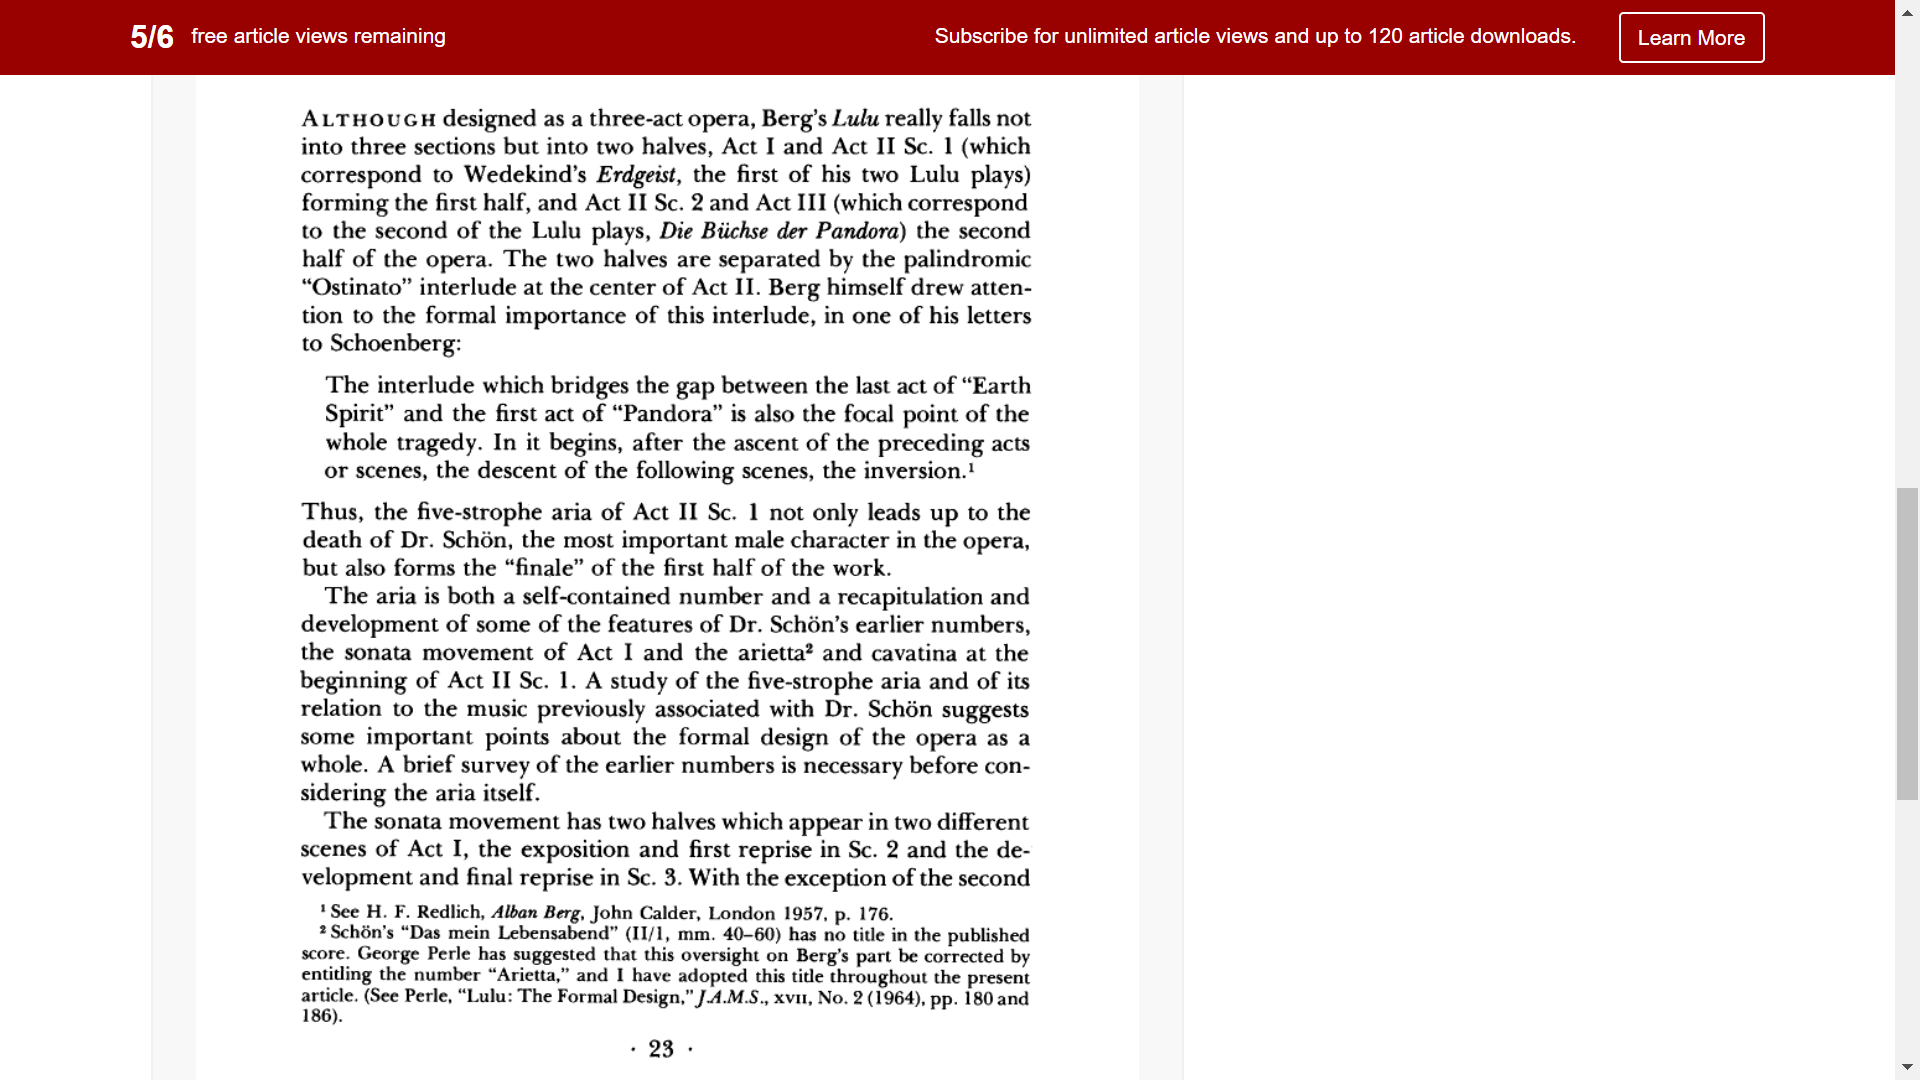
\includegraphics[width=12.1cm]{1.png}
		\end{center}
		
		\emph{3. La serie ser\'a expuesta en cualquiera de sus aspectos lineales: original, inversi\'on, retrogradaci\'on de la original y retrogradaci\'on de la inversi\'on.}
		 
		\emph{4. La serie puede usarse en sus cuatro aspectos desde cualquier nota de la escala.}
		
		Los dos \'ultimos postulados ampl\'ian los recursos compositivos al admitir la transformaci\'on de la serie original mediante \emph{inversi\'on}, \emph{retrogradaci\'on}, \emph{inversi\'on retr\'ograda} y \emph{transposici\'on}\footnote{No confundir con un 2-ciclo. Una transposici\'on musical se corresponde con una traslaci\'on matem\'atica.}. El compositor puede utilizar cualquiera de las transformaciones de una serie al componer su obra dodecaf\'onica. El conjunto de series que puede utilizar, que viene dado por la serie original y todas sus posibles transformaciones, se conoce como \emph{espectro serial}. \cite{dominguez}
		
	\subsection{Las transformaciones de una serie}
		\label{transPsi}
		Transformar una serie es matem\'aticamente equivalente a aplicar una funci\'on sobre la serie, y que asocie esa permutaci\'on a la permutaci\'on transformada. Por tanto, cualquier funci\'on transformativa $\Psi$ se aplica sobre el conjunto de las permutaciones, S$_{12}$.
		
	\subsubsection{Transposiciones}
		La \emph{transposici\'on}, mencionada en el cuarto postulado, consiste en subir o bajar la serie original un n\'umero determinado de semitonos. Por tanto, no se modifican los intervalos entre las notas, sino solamente la altura a la que est\'a la serie. Ya que consideraremos todas las octavas equivalentes, debemos trabajar m\'odulo 12. 
		
		La serie transportada k semitonos (con k constante),
		
		$\mbox{T}^{{\mbox{k}}}(\sigma)$, se construye sumando k a $\sigma$ (mod. 12):
		\[\mbox{T}^{{\mbox{k}}}(\sigma(m))=\sigma(m)+{\mbox{k}}\]		
		{\[
		\mbox{T}^{{\mbox{k}}}=
		\left(\begin{array}{*{7}c}
			0&1&2&&9&10&11\\
			\sigma(0)+{\mbox{k}}&\sigma(1)+{\mbox{k}}&\sigma(2)+{\mbox{k}}&
			\cdots&
			\sigma(9)+{\mbox{k}}&\sigma(10)+{\mbox{k}}&\sigma(11)+{\mbox{k}}\\
		\end{array}\right)
		\]}
		
		A su vez, T$^{\mbox{k}}$ se forma al componer k transposiciones de 1 semitono: $\mbox{T}^{\mbox{k}}=\mbox{T}^1\circ\mbox{T}^1\circ\ldots\circ\mbox{T}^1$, k veces. Debido a que k es en realidad el exponente en la potencia de T, se coloca este n\'umero como super\'indice.
		
		Hist\'oricamente, la notaci\'on $\Psi_{\mbox{k}}$, $\Psi^{\mbox{k}}$ o $\Psi({\mbox{k}})$ se ha usado en sustituci\'on de la composici\'on de la transposici\'on T$^{\mbox{k}}$ y otra funci\'on $\Psi$, en el respectivo orden: $\Psi^{\mbox{k}}=\Psi \circ \mbox{T}^{\mbox{k}} = \Psi(\mbox{T}^{\mbox{k}})$. Sin embargo, esta notaci\'on es especialmente ambigua y confusa, sobre todo al trabajar con funciones no conmutativas. Por ello, es preferible ce\~nirse a la notaci\'on estrictamente matem\'atica; es decir, a la composici\'on de funciones, aun omitiendo $\circ$: \cancel{$\Psi_{\mbox{k}}$}, \cancel{$\Psi^{\mbox{k}}$}, \cancel{$\Psi({\mbox{k}})$} $arrow \Psi\mbox{T}^{\mbox{k}}$
		
		Una posible serie transportada sobre la permutaci\'on $\sigma$ de la Suite para piano Op. 25, con k $= 6$, es la siguiente serie T$^6$:
		\[\mbox{T}^6=\drow{10,11,1,7,0,9,2,8,5,6,3,4}\]	
		\begin{center}
			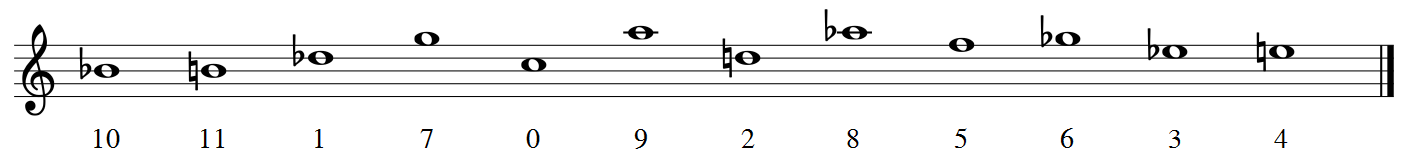
\includegraphics[width=12.1cm]{2.png}
		\end{center}
		
	\subsubsection{Retrogradaci\'on}
		La \emph{retrogradaci\'on} consiste en leer la serie original desde la nota final hacia atr\'as, es decir, aplicar a la serie una simetr\'ia especular. De este modo, la primera nota ir\'a al \'ultimo puesto, la segunda al pen\'ultimo, y as\'i sucesivamente.
		
		La serie retr\'ograda se construye de esta forma:
		\[\mbox{R}(\sigma(m))=\sigma(-1-m)\]
		\[{\mbox{R}=\drow{\sigma(11),\sigma(10),\sigma(9),\sigma(8),\sigma(7),\sigma(6),\sigma(5),\sigma(4),\sigma(3),\sigma(2),\sigma(1),\sigma(0)}}\]
			
		La serie retr\'ograda sobre la permutaci\'on $\sigma$ de la Suite Op. 25 es la siguiente serie R:	
		\[\mbox{R}=\drow{10,9,0,11,2,8,3,6,1,7,5,4}\]		
		\begin{center}
			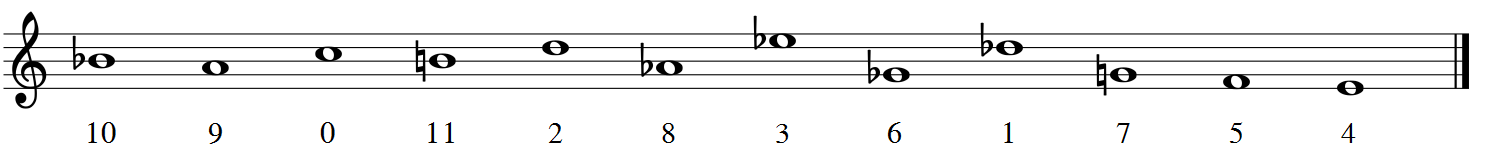
\includegraphics[width=12.1cm]{3.png}
		\end{center}
		
	\subsubsection{Inversi\'on}
		La \emph{inversi\'on} consiste en cambiar la direcci\'on --de ascendente a descendente, y viceversa-- de los intervalos entre cada nota de la serie. Si el primer intervalo en la serie original $\sigma$ es de $+k$, el primer intervalo en la serie invertida I ser\'a de $-k$ (mod. 12), por lo que debemos cambiar el signo de $\sigma$ para construir I. Adem\'as, queremos que la primera nota de ambas series, I(0) y $\sigma$(0), coincidan, as\'i que debemos transportar la serie ($-\sigma$) un n\'umero $\lambda$ de semitonos para que esta condici\'on se cumpla:
		\begin{align*}
		\mbox{I}(0)=-\sigma(0)+\lambda&=\sigma(0)\\
		\Longrightarrow \lambda&=2\sigma(0)
		\end{align*}
		Por tanto, la serie invertida se construye de esta forma:
		\[\mbox{I}(\sigma(m))=-\sigma(m)+2\sigma(0)\]
		
		\[\mbox{I}=\left(\begin{matrix}0&1&2&&10&11\\\sigma(0)&-\sigma(1)+2\sigma(0)&-\sigma(2)+2\sigma(0)&\ldots&-\sigma(10)+2\sigma(0)&-\sigma(11)+2\sigma(0)\\\end{matrix}\right)\]
		
		La serie invertida sobre la permutaci\'on $\sigma$ de la Suite Op. 25 es la siguiente serie I:
		\[\mbox{I}=\drow{4,3,1,7,2,5,0,6,9,8,11,10}\]		
		\begin{center}
			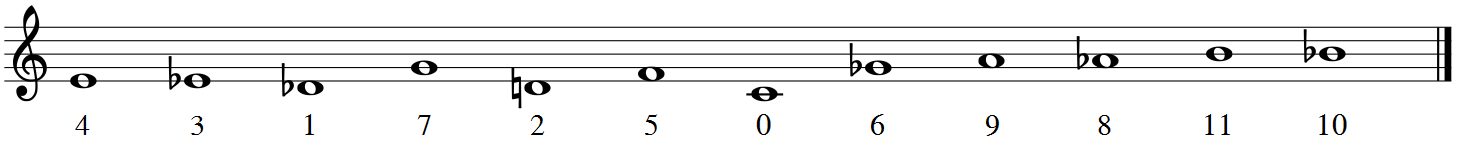
\includegraphics[width=12.1cm]{4.png}
		\end{center}
				
		En total, obtendremos 48 series -- aunque no obligatoriamente distintas entre s\'i -- pertenecientes a un solo espectro serial. Hay 12 series originales sobre cada una de las doce notas, 12 series retr\'ogradas, 12 invertidas y 12 series sobre las que se aplica tanto la retrogradaci\'on como la inversi\'on. A continuaci\'on se muestra la sintaxis simple junto a la matem\'atica:
		
		\begin{multicols}{2}
			\underline{Sintaxis simple}
			
			T$_0$, T$_1$, T$_2$\ldots
			
			R$_0$, R$_1$, R$_2$\ldots
			
			I$_0$, I$_1$, I$_2$\ldots
			
			IR$_0$, IR$_1$, IR$_2$\ldots
			
			\underline{Sintaxis matem\'atica}
			
			T$^0$, T$^1$, T$^2$\ldots
			
			R, RT$^1$, RT$^2$\ldots
			
			I, IT$^1$, IT$^2$\ldots
			
			IR, IRT$^1$, IRT$^2$\ldots
		\end{multicols}
	
	\subsection{Matrices dodecaf\'onicas}
		
		Dada una serie, su matriz dodecaf\'onica es una representaci\'on visual de su espectro serial; es decir, del conjunto de series derivadas de esa serie. El espectro serial es todo el material compositivo sonoro del que se dispone para la composici\'on de una obra dodecaf\'onica. Al poder ordenar y disponer la informaci\'on en una tabla, el compositor puede acceder a toda ella al mismo tiempo sin tener que calcular cada serie individualmente.		
		
		La matriz se lee en la direcci\'on en la que aparece el nombre de la serie. Las series T se leen de izquierda a derecha, mientras que las series R de derecha a izquierda. Las series I se leen de arriba a abajo y las IR/RI de abajo a arriba.
		
		He creado un programa que devuelve en formato \LaTeX{} la matriz correspondiente a cualquier serie dodecaf\'onica que se introduzca en teclado, adem\'as de producir la nomenclatura simple para cada serie. El c\'odigo, escrito en C++, %est\'a incluido en el Anexo \ref{app:matrices}, p\'agina \pageref{app:matrices}.
		se puede encontrar en el enlace \url{https://gitlab.com/dodecafonismo/cppmatrices}.
		
		A continuaci\'on, se incluye la matriz dodecaf\'onica de la serie P de la Suite Op. 25 de Schoenberg. Mientras que la mayor\'ia de tablas tienen dos filas inferiores, que se corresponden con las distintas nomenclaturas de RI e IR para una misma serie -- ya que normalmente no conmutan --, en la matriz de la serie P s\'i coinciden%, como se mencionar\'a en el apartado \ref{conmut}
		.
		
		{$\begin{array}{l|cccccccccccc|r}
		&\mbox{I}_{0}&\mbox{I}_{1}&\mbox{I}_{3}&\mbox{I}_{9}&\mbox{I}_{2}&\mbox{I}_{11}&\mbox{I}_{4}&\mbox{I}_{10}&\mbox{I}_{7}&\mbox{I}_{8}&\mbox{I}_{5}&\mbox{I}_{6}&\\
		\hline
		\mbox{T}_{0}&4&5&7&1&6&3&8&2&11&0&9&10&\mbox{R}_{0}\\
		\mbox{T}_{11}&3&4&6&0&5&2&7&1&10&11&8&9&\mbox{R}_{11}\\
		\mbox{T}_{9}&1&2&4&10&3&0&5&11&8&9&6&7&\mbox{R}_{9}\\
		\mbox{T}_{3}&7&8&10&4&9&6&11&5&2&3&0&1&\mbox{R}_{3}\\
		\mbox{T}_{10}&2&3&5&11&4&1&6&0&9&10&7&8&\mbox{R}_{10}\\
		\mbox{T}_{1}&5&6&8&2&7&4&9&3&0&1&10&11&\mbox{R}_{1}\\
		\mbox{T}_{8}&0&1&3&9&2&11&4&10&7&8&5&6&\mbox{R}_{8}\\
		\mbox{T}_{2}&6&7&9&3&8&5&10&4&1&2&11&0&\mbox{R}_{2}\\
		\mbox{T}_{5}&9&10&0&6&11&8&1&7&4&5&2&3&\mbox{R}_{5}\\
		\mbox{T}_{4}&8&9&11&5&10&7&0&6&3&4&1&2&\mbox{R}_{4}\\
		\mbox{T}_{7}&11&0&2&8&1&10&3&9&6&7&4&5&\mbox{R}_{7}\\
		\mbox{T}_{6}&10&11&1&7&0&9&2&8&5&6&3&4&\mbox{R}_{6}\\
		\hline
		&\mbox{IR}_{0}&\mbox{IR}_{1}&\mbox{IR}_{3}&\mbox{IR}_{9}&\mbox{IR}_{2}&\mbox{IR}_{11}&\mbox{IR}_{4}&\mbox{IR}_{10}&\mbox{IR}_{7}&\mbox{IR}_{8}&\mbox{IR}_{5}&\mbox{IR}_{6}&\\
		\hline
		&\mbox{RI}_{0}&\mbox{RI}_{1}&\mbox{RI}_{3}&\mbox{RI}_{9}&\mbox{RI}_{2}&\mbox{RI}_{11}&\mbox{RI}_{4}&\mbox{RI}_{10}&\mbox{RI}_{7}&\mbox{RI}_{8}&\mbox{RI}_{5}&\mbox{RI}_{6}&
		\end{array}$}
	
		Por otro lado, he escrito otro programa en el propio lenguaje \LaTeX{} que crea esta misma tabla con el comando \verb|\dmatrix|, y tiene cualquier serie como argumento: \verb|\dmatrix{4,5,7,1,6,3,8,2,11,0,9,10}|. %El c\'odigo se encuentra en el Anexo \ref{app:latex}, p\'agina \pageref{app:latex1}. 
		El c\'odigo se encuentra en el paquete de \LaTeX{} \texttt{ddphonism}, incluido en el enlace  \url{https://gitlab.com/dodecafonismo/ddphonism}.
		La tabla aparece sin el orlado de nomenclaturas:
		\dmatrix{4,5,7,1,6,3,8,2,11,0,9,10}
		
		Tambi\'en he creado una p\'agina interactiva que genera matrices de cualquier serie para cualquier longitud serial, adem\'as de generar series aleatorias. Permite escoger entre dos numeraciones y dos nomenclaturas. Est\'a escrita en Elm y el c\'odigo puede encontrarse en \url{https://gitlab.com/dodecafonismo/matrices}.
		
%			\qrcode{https://matrices.netlify.com/}
			
			En este enlace se encuentra la aplicaci\'on web. Sus instrucciones de uso se encuentran al final de la p\'agina: \url{https://matrices.netlify.com/}.